\documentclass[15pt]{article}
\usepackage[utf8]{inputenc}
\pagestyle{plain}
\usepackage{amsmath, amssymb, amsfonts, amsthm, mathtools, mathrsfs}
\usepackage[
top    = 2.75cm,
bottom = 2.55cm,
left   = 3.00cm,
right  = 3.00cm]{geometry}
\usepackage{graphicx}
\usepackage{xcolor}
\usepackage{listings}
\usepackage{xcolor}
\lstset { %
    language=C++,
    backgroundcolor=\color{black!5}, % set backgroundcolor
    basicstyle=\footnotesize,% basic font setting
}

% \pagecolor[RGB]{18,18,18} %blackish
% \color[rgb]{0.9, 0.9, 0.9} %greyish

\usepackage{bm}
\usepackage{physics}
\usepackage{hyperref}
\usepackage{titlesec}
\usepackage{tocloft}
\usepackage{caption}
\usepackage{subcaption}
\usepackage[none]{tocbibind}
\usepackage{float}
\usepackage{fancyhdr}

\titleformat*{\subsection}{\normalfont}
\graphicspath{ {./CS101 images/} }
\definecolor{- }{RGB}{252,107,63}
\definecolor{v}{RGB}{112,100,240}
\setcounter{secnumdepth}{5}
\setcounter{tocdepth}{1}

\pagestyle{fancy}
\fancyhf{}
\renewcommand{\headrulewidth}{0pt}
\renewcommand{\footrulewidth}{0.4pt}
\fancyfoot[R]{ADI}
\fancyfoot[L]{\thepage}

\renewcommand{\b}[1]{\begin{#1}}
\newcommand{\e}[1]{\end{#1}}
\renewcommand{\i}{\item{}}
\newcommand{\tb}[1]{\textbf{#1}}
\renewcommand{\thefigure}{}
\renewcommand{\cfttoctitlefont}{\Huge}

\b{document}
   \b{center}
       \vspace*{12cm}
       \tb{{\Huge CS101 Short Notes}}
       
       \vspace{0.9cm}
       \tb{\LARGE Aditya Byju}
            
       \vspace{0.5cm}
       \large {\tb{Course Professor:} Prof. Bhaskaran Raman \\\& Prof. Kameswari Chebrolu\\
       \tb{Ref:} Prof's slides\\
       There is an easy way and a hard way\\The hard part is finding the easy way}
       
       \vspace{0.5cm}
       \tb{Computer Programming and Utilization}
       
       \vspace{0.5cm}
       September 2021
            
       \vspace{0.8cm}
    \e{center}
\thispagestyle{empty}

\newpage
\tableofcontents
\addtocontents{toc}{\vspace{0.2cm}}

\newpage
\phantomsection
\section*{\color{- }Basic C++}
\addcontentsline{toc}{section}{\large\color{- }Basic C++}

\b{itemize}
    \i {\color{v}Linux} is open source and is developed by Linux community of developers. {\color{v}Unix} was developed by AT\&T Bell labs and is not open source. Linux is free to use. Unix is licensed OS.
    \i Why use Unix command-line?
    \begin{itemize}
        \item {\color{v}Windows GUI:} uses pre-programmed interface - set of possible actions are pre-decided
        \item {\color{v}Command-line shell:} a prog. (scripting) language - we can use pre-written programs and compose new scripts
    \end{itemize}
    \i Some commands:
    \begin{itemize}
        \item {\color{v}ls:} list files or directories
        \item {\color{v}ls -a:} list all files or directories (hidden too)
        \item {\color{v}pwd:} prints current working directory 
        \item {\color{v}cd:} change   directory
        \item {\color{v}mkdir:} make directory
        \item {\color{v}rmdir:} remove directory
        \item {\color{v}cat:} show content of given filename
        \item {\color{v}less:} show content of given filename in a scrollable format
        \item {\color{v}cp:} copy file from source to destination
        \item {\color{v}mv:} move file from source to destination
        \item {\color{v}rm:} remove files, directories and links
        \item {\color{v}emacs:} text editor
        \item {\color{v}ps:} to list the processes
        \item {\color{v}kill:} to kill a process
        \item {\color{v}tar:} to zip files and folders
        \item {\color{v}grep:} used for finding patterns within files
        \item {\color{v}man:} manual of a particular command
    \end{itemize}
    \i The Unix File System:
    \begin{itemize}
        \item Three kinds of permissions: {\color{v}read, write, execute}
        \item Three levels of access control: {\color{v}user, group, all}
    \end{itemize}
    \i {\color{v}program} - a precise description of the calculations we want the computer to perform 
    \i The C++ programming language was designed by Bjarne Stroustrup, in the 1980s. It evolved out of C programming language.
    \i {\color{v}syntax} - grammatical rules indicating how commands must be written
    \i {\color{v}control flow} - the order in which statements get executed
    \i {\color{v}ASCII} - American Standard Code for Information Interchange. `a'$=97, $ `b'$=98,\ldots$
    \i {\color{v}algorithm} - a precise description of the operations needed to solve a problem
    \i Single precision float (32 bits):
    \begin{itemize}
        \item 1 bit for sign of significand/mantissa
        \item 23 bits for mantissa itself
        \item 8 bits for exponent (signed)
    \end{itemize}
    \i Double precision float (64 bits):
    \begin{itemize}
        \item 1 bit for sign of significand/mantissa
        \item 52 bits for mantissa itself
        \item 11 bits for exponent (signed)
    \end{itemize}
    \i Signed numbers are represented by two’s complement
    \i Real numbers are represented by IEEE 754 standard (float, double)
    \begin{figure}[H]
    \centering
    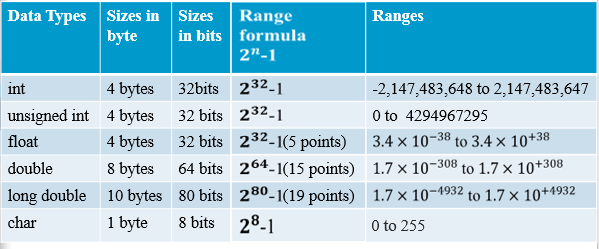
\includegraphics[width=14cm]{Variable Types.png}
    \caption{Variable Types and Ranges}
    \end{figure}
    \i Compiler translates the C++ program to a Machine language program
    \i To print newline, use endl
    \i Multiplication, division have same precedence.  Addition, subtraction have same precedence. Operators of same precedence will be evaluated left to right.
    \i Initialization happens left to right
    \i x \% y evaluates to the remainder when x is divided by y. x, y must be integer expressions.
    \i Code inside \{\} is called a block
    \i All variables defined in a block are destroyed every time control  reaches the end of the block
    \i  Variables defined outside a block can be used inside the block, if no variable of the same name is defined inside the block. If a variable of the same name is defined, then from the point of definition to the end of the block, the newly defined variable gets used. The new variable is said to “shadow” the old variable. The region of the program where a variable defined in a particular definition can be used is said to be the scope of the definition.
    \i Variables are regions of memory which can store values
    \i 'consequent' is a C++ statement
    \i Flowchart is a pictorial representation of a program. Diamond shaped boxes are used for condition checks.
    \i AND: \&\&
    \i OR: $\mid\mid$
    \i NOT: !
    \i ! has higher precedence than \&\& which has higher precedence than $\mid\mid$
    \i C++ has data type bool into which values of conditions can be stored
    \i If break appears inside a while statement which is itself nested inside another while, then then the inner statement is terminated. The continue statement enables us to skip the rest of the iteration.
    \i Form of for statement: for(initialization; condition; update) body
    \i In the case of for statement new variables can be defined in initialization. These variables are accessible inside the loop body, including condition and update, but not outside. The variable which is initialized is called the control variable of the for statement. Leaving the initialization part of the for statement empty is allowed.
    \i m, n, have the same common divisors as m-n, n. The largest divisor of m,n is also the largest divisor of m-n,n. To find GCD(m,n), we might as well find GCD(n, m-n).
    \i Euclid’s theorem: Let $m, n>0$ be positive integers. If n divides m then GCD(m,n) = n. Otherwise GCD(m,n) = GCD(m\%n, n).
    \i In Taylor series error using first $k$ terms $\leq |(k+1)^{th}$ term$|$
    \i In mathematics, the bisection method is a root-finding method that applies to any continuous function for which one knows two values with opposite signs.
    \i In order to perform numerical integration we just need to be able to evaluate the given function at an arbitrary point.
    \i The Newton-Raphson method begins with an initial estimate of the root, denoted $x_0\neq x_r$, and uses the tangent of f(x) at x0 to improve on the estimate of the root. In particular, the improvement, denoted x1, is obtained from determining where the line tangent to f(x) at x0 crosses the x-axis. This represents a single iteration of the Newton-Raphson method
    \i A number is said to be perfect if it is the sum of all its divisors smaller than itself
    \i Area allocated in memory where a function will have its variables is called the activation frame of that function
    \i Calling program will refer to the variables in its activation frame. Called program will refer to the variables in its activation frame.
    \i Function definition must appear before any call to it in the program file
    \i Main program is also a function
    \i If a function does not return a value its return type is void
    \i Function is a piece of code which takes the responsibility of getting something done
    \i Preconditions are certain properties that the arguments of a function satisfy. What is promised about the state of the computer after the function finishes execution is called postcondition.
    \i Variable names can be the same in the main program and in the function
    \i A function is like an independent program except that it gets some values (arguments) from the calling program, and returns results to the calling program
    \i \& before the name of the parameter does not allocate space for the parameter, but instead just uses the variable from the calling program. Such parameters are called reference parameters. If a certain parameter is a reference parameter, then the corresponding argument is said to be “passed by reference”.
    \i If we want to return more than one result we can do so by using a reference parameter.
    \i A pointer is a variable that can store addresses
    \i The operator \& can be used to get the address of a variable. The same \& is used to mark reference parameters; but the meaning will be clear from the context.
    \i Customarily, addresses get printed in hexadecimal radix, i.e. they will consist of a sequence of hexadecimal digits prefixed by “0x”
    \i Variable for storing addresses of variables of type int : int *v;
    \i The * is not to be read as multiplication. Think of it as (int*) v; where int* means the type: “address of int”.
    \i In general, to create a variable w to store addresses of variables of type T, write: T* w;
    \i Recursion is the phenomenon of a function calling itself. There is no circularity if the arguments to the new call are different from the arguments in the original call. Each call executes in its own activation frame.
    \i Recursion often produces compact, elegant programs. Recursive programs might be slightly slower because they need to create activation frames etc.
    \i Designing a recursive algorithm:
    \begin{itemize}
        \item attempt to solve the given problem instance by constructing and solving smaller instances of the same type
        \item solve the simplest instances directly
    \end{itemize}
    \i Top level recursive call: the call made from the main program, or the first call made to the recursive function
    \i Level 1 recursive calls: calls made directly while executing the top level call
    \i Base cases: input values for which the top level call returns without recursing
    \i Preconditions: valid values for inputs
    \i Problem size: something indicative of the amount of e=work needed to find the solution. Needs to be chosen creatively.
    \i To check if a recursive function is correct we should check:
    \begin{itemize}
        \item there are base cases and correct results are obtained for the base cases
        \item the level 1 recursive calls satisfy the preconditions
        \item the problem size reduces but cannot reduce indefinitely
        \item if the level 1 calls work correctly, whether the top level call works correctly
    \end{itemize}
    \i The execution of any recursive program can be visualized by drawing its “Execution tree” or its “Recursion tree”
    \i Fibonacci sequence are the Virahanka numbers
    \i The natural recursive algorithm might be very slow. By examining what the algorithm does, we might be able to discover a better algorithm.
    \i The function main is allowed not to have a return statement
    \i If code in a file F calls a function f, it must be declared inside F, textually before any call to it. A function definition is a declaration. A function declaration is essentially just the definition without the body. Other names for declaration are "Signature" and "Prototype".
    \i If a file contains a call to a function but does not contain its definition, then it can only be partially compiled into an object module. To get an executable program, all the object modules containing all called functions must be linked together.
    \i Tedious to remember what declarations to include in each file. Instead, we can put all declarations into a header file, and "include" the header file into every file. Header files customarily have the suffix .h or .hpp, or no suffix.
    \i It is acceptable if we have both a declaration and then the definition of a function in the same file
    \i If header file is mentioned in `` ", it is picked up from the current directory. If it is mentioned in $<>$, it is picked up from some standard place.
    \i Namespace = catalog of names. The ``full name" of a function defined in a namespace N is N::f.
    \i Defining a namespace:
    \begin{lstlisting}
    namespace N{
    declarations/definition of names
    }
    \end{lstlisting}
    \i You can add more names to a namespace N simply by writing namespace n\{\} again. A name g defined without putting it inside a namespace is said to belong to the global namespace. Its fullname is ::g.
    \i You will be allowed to use any name from N without having to write N:: before it if you put the following line at the top of your program: using namespace n;
    \i Some initial lines of code in C++:
    \begin{lstlisting}
    #include <iostream>
    #include <cmath>
    using namespace std;
    \end{lstlisting}
    The names cin, cout, endl are defined in the namespace std, in the standard header file iostream. The header file cmath includes math functions such as sqrt, sin, abs.
    \i To pass a function h to another function B the type of h is: std::function$<$return-type(parameter1-type, \ldots)$>$. Must include header file <functional> in order to use this feature.
    \i Lambda expression = an expression which represents a (nameless) function. General form: [](parameter list){body}.
    \i You can pass arguments to the function and it is evaluated like an ordinary function call: [](double x){return x*x – 2;}(3.5)
    \i Return type is not stated explicitly. It is inferred by the C++ compiler. In case it is not possible to infer the type, you can specify it explicitly too: [](parameter-list)->return type {body}
    \i In lambda expressions you can capture outside variables by putting a comma seperated list in [], i.e., lambda expressions can also capture the values of variables defined in the function in which the lambda expression appears.
    \i One or more parameters occurring at the end of the parameter list can be given default values. Note that if you want to specify a default value for the $r^{th}$ parameter, you must specify a default value for all subsequent parameters as well.
    \i C++ allows you to define multiple functions with the same name, provided they have different argument lists
    \i General form of an array: data-type array-name[size];
    \i Indexing into an array happens very fast, independent of how many elements are present in the array
    \i Array name = address of allocated region = address of $0^{th}$ array element. Type of array name: int *. Array name is a pointer, but its value cannot be changed.
    \i [] is a binary operator. aname[index] means that the variable is stored at aname + S*index, where S = size of a single element of the type aname points to. The computer does a multiplicatin and addition to find the position of the element in memory. Note that only a single multiplication and addition is done, however large the array is.
    \i Some programming languages prevent index out of range by explicitly checking. Index checking is not done in C++, because it takes extra work and C++ designers believe that it is the programmer's job to ensure that the index is in range.
    \i In a function call, array elements are not copied. If the function modifies the elements, then the modification will be seen in the calling program.
    \i The interesting part is the [] operator: given the address of an array and an index it can get us to the corresponding element, even if the address belongs to a different activation frame
    \i An alternate syntax is also allowed: int avg(double M[], int n){\ldots}. In this double M[] is synonymous with double *M, but slightly more indicative that we expect M to be an array name, and not just any old pointer.
    \i The selection sort algorithm sorts an array by repeatedly finding the minimum element (considering ascending order) from unsorted part and putting it at the beginning. The algorithm maintains two subarrays in a given array: The subarray which is already sorted, and the remaining subarray which is unsorted. In every iteration of selection sort, the minimum element (considering ascending order) from the unsorted subarray is picked and moved to the sorted subarray. 
    \i Time complexity of selection sort: O($n^2$), where $n$ is the number of elements being sorted
    \i char type meant to store single letter. Array of char can be used to store sequences of letters.
    \i Standard protocol inherited from the C language for char:
    \begin{itemize}
        \item store characters in the string in the array starting from element 0
        \item after all the characters are stored, store the character `\textbackslash 0'
        \item `\textbackslash 0' = ``sentinel" = character whose ASCII value is 0. ``null" character.
        \item key idea: ``Everything until `\textbackslash 0' is a part of the string, not what comes later"
        \item no need to explicitly store the length of the string
    \end{itemize}
    \i Safe way to read into a char array: cin.getline(charArrayName, n);
    \i For 2-dimensional arrays values picked from the initialization list in row major order
    \i When passing 2-dimensional arrays to functions, C++ requires to specify the number of columns as a fixed number at the time of writing the function. This is a C++ language limitation. 
    \i We can call main function with a more elaborate signature as shown:
    \begin{lstlisting}
    namespace N{
    declarations/definition of names
    }
    \end{lstlisting}
    argc: gives the number of ``words" typed on the command line. Each element of argv is a pointer to each word typed on the command line.
    \i Linear search is a sequential searching algorithm where we start from one end and check every element of the list until the desired element is found. It is the simplest searching algorithm. Time complexity: O(n).
    \i Binary Search is a searching algorithm used in a sorted array by repeatedly dividing the search interval in half. The idea of binary search is to use the information that the array is sorted and reduce the time complexity to O(Log(n)). 
    \i If you are likely to search an array frequently, first sort it, then binary search. The time to sort the array will be compensated by the time saved in subsequent searches.
    \i Merge sort divides the input array into two halves, calls itself for the two halves, and then it merges the two sorted halves. Time complexity: O(n Log(n))
    \i Structure is a group/supervariable which is a collection of all information about an entity
    \i Members of a structure are the variables in the collection. Each structure has a type which defines what variables there will be in the collection. You can define a structure type foe each type of entity that you want to represent on the computer - ``Programmer defined type"
    \i General form of struct:
    \begin{lstlisting}
    struct structure-type{
    member1-type member1-name;
    member2-type member2-name;
    ...
    }; // Don't forget the semicolon!
    \end{lstlisting}
    \i int, char, double etc. are primitive data types
    \i One structure can contain another
    \i Main program is at high level
    \i (*x).y is same as x $-\hspace{-0.1cm}>$ y
    \i NULL is a keyword in C++. It can be assigned to any pointer, to indicate that the pointer does not point to anything meaningful.
    \i Functions inside the structure which is used to access the attributes are called member functions
    \i The member function call can modify the members in the receiver, since the receiver is implicitly passed by reference
    \i The only difference between a structure and a class is that structure members have public access by default and class members have private access by default
    \i An Object is an instance of a Class
    \i In C++, the programmer may define a special member function called a constructor. The constructor is called whenever an instance of the struct is created. A constructor has the same name as the struct, and no return type. The code inside the constructor can perform initializations of members. Constructor can take arguments. You can have many constructors, provided they have different signatures.
    \i C++ defines a constructor which takes no arguments, and does nothing if and only if you do not define a constructor. A constructor that does not take arguments (defined by you or C++) is called a default constructor.
    \i If a member is itself a struct, its constructor is called first
    \i Operator overloading: consider x@y where @ is any ``infix" operator, C++ treats this as: x.operator@(y). operator@ must be a member function.
    \i It is possible to restrict access to members or member functions of a struct. This is called access control. Members declared private can only be accessed inside the definition of the struct.
    \i Typical strategy: declare all data members to be private, and some subset of function members to be public
    \i public:, private: are access specifiers. An access specifier applies to all members defined following it, until another specifier is given.
    \i cin, cout are objects of class istream, ostream respectively. $<<,>>$: operators defined for the objects of these classes.
    \i You must include header file $<$fstream$>$ to use ifstream and ofstream
    \i Example of file i/o:
    \begin{lstlisting}
    #include <fstream>
    #include <iostream>
    int main(){
     ifstream infile("f1.txt");
     ofstream outfile("f2.txt");
     int v;
     infile >> v;
     outfile << v<<endl;
     }
    \end{lstlisting}
    \i object, structure variable, instance of a class: synonyms
    \i Object oriented programming: metholodogy for programming design - 
    \begin{itemize}
        \item suggests that real life entities be modelled using structs/classes
        \item recommends member functions be used for performing operations
        \item recommends that data members be hidden
    \end{itemize}
    \i If you do not define any member functions, C++ defines folloeing member functions:
    \begin{itemize}
        \item constructor
        \item assignment operator
        \item copy constructor
        \item destructor
    \end{itemize}
    If you define any of these, your definitions override.
    \i For nested structures, first constructors of members are called, then constructor of outer object
    \i Assignment operator: if you do not define an assignment operator, operator=, C++ defines one. This predefined assignment operator simply does member by member copy.
    \i Copy constructor: when you pass a structure to a function (by value), a copy needs to be made. This is done by a function called the copy constructor. C++ provides a predefined copy constructor. It copies member by member.
    \i Destructor: when an object goes out of scope, or is deleted, a destructor member function gets called. Predefined destructor does nothing.
    \i In automatic variables, memory allocation/deallocation happens automatically
    \i ``Heap” memory, also known as ``dynamic” memory, is an alternative to local stack memory. Local memory is quite automatic. Local variables are allocated automatically when a function is called, and they are deallocated automatically when the function exits. Heap memory is different in every way.
    \i It is possible to explicitly request that, memory for a certain variable be allocated in the heap. When there is no more use for the allocated memory, the program must explicitly return the memory to the heap. After the memory is returned, it can be used to satisfy other memory allocation requests in the future. Neither allocation, nor deallocation of this memory is automatic. No deallocation happens just because a block is exited by the control.
    \i The standard library classes use heap memory
    \i Syntax for allocating heap memory: new T (T = typename). Memory for storing one variable of type T is allocated on the heap. new T returns address of allocated memory. After the memory is no longer needed, it must be returned by executing delete. An example:
    \begin{lstlisting}
    class Book{
     char title[100];
     double price;
    };
    Book *bptr;
    bptr = new Book;
    bptr-\hspace{-0.2cm}>price = 399;
    ...
    delete bptr;
    \end{lstlisting}
    \i Allocating arrays on the heap:
    \begin{lstlisting}
    char* cptr;
    cptr = new char[10]; 
    // allocates array of length 10.
    // array can be accessed as usual 
    // cptr[0],...,cptr[9]
    delete[] cptr; 
    // When not needed. 
    // Note: delete[] not delete
    \end{lstlisting}
    \i Storing many names:
    \begin{lstlisting}
    char *names[100]; // array of pointers to char
    for(int i=0; i<100; i++){
     char buffer[80]; cin >> buffer;
     int L = length(buffer)+1; // length: returns no of chars till `\0' 
     // +1 so that we can append `\0'.
     names[i] = new char[L];
     for(int j=0;j<L;j++)
     names[i][j] = buffer[j];
    }
    \end{lstlisting}
    \i Managing heap memory is tricky and prone to errors:
    \begin{itemize}
        \item forgetting to deallocate (delete) memory
        \item referring to memory that has been deallocated (``dangling reference")
        \item destroying the only pointer to memory allocated on the heap before it is deallocated (``memory leak")
    \end{itemize}
    \i Simple strategy for preventing memory leaks:
    \begin{itemize}
        \item suppose a certain pointer variable, ptr, is the only variable that contains the address of a variable allocated on the heap
        \item we must not store anything into ptr and destroy its contents
        \item when ptr is about to go out of scope, (control exits the block in which ptr is defined) we must execute delete ptr;
    \end{itemize}
    \i For preventing dangling references, ensure that at all times, each variable on the heap will be pointed to only by one pointer
    \i this is a C++ keyword. Inside a member function, this is a pointer to the receiver. *this would mean the receiver itself.
    \i #include <string> is needed to use the string class
    \i #include <vector> is needed to use the vector class
    \i Use vectors, not arrays!
    \i General form of maps: map$<$indextype, valuetype$>$ mapname;
    
    
    
    
    

\e{itemize}



\e{document}
